\section{Graph theory}
Because of the network structure of FPGAs, it is easy to model them as graphs. If we model FPGA components as combinations of vertices and connections, we have a complete representation of an FPGA suitable for graph algorithms. Let us suppose that we find a subgraph embedding of a graph representation of a virtual FPGA model in a graph representation of a concrete FPGA model. Then, by copying configurations from components in the virtual FPGA model to their concrete mapping we would have an emulation function. This could entail changing some bits if, for example, the second output of a virtual LUT is mapped the the first output of the concrete LUT and vica versa. While virtual components may also be emulated by structures of multiple concrete components connected in specific ways, we deem finding such emulations out of scope for this research.

The graph theoretic name for finding these embeddings is subgraph isomorphism. It is an NP-complete problem\cite{cook} with many algorithms explored. The problem with using an approach of subgraph isomorphism is, however, that many possible emulations cannot be found. For example, a concrete FPGA may have much more configurable routing switches than an virtual FPGA. A subgraph isomorphism algorithm would in this case not find an emulation, even though one is technically possible by configuring some routing switches to function as wires.

A variant of subgraph isomorphism is (vertex disjoint) subgraph homeomorphism. In this problem, intermediate vertices are allowed in the embedding on the target-graph side. This means that the embedding consists of a vertex-to-vertex mapping and an edge-to-path mapping.


\begin{defn}[graph]
A graph is a tuple $(V, E, L)$ where $V$ is a set of vertices, $E$ is a multiset of directed edges such that each edge $e \in E \to e \in (V \times V)$ and $L: (V \to \mathbb{P}(\lambda))$ is a multilabelling function where $\lambda$ is a finite alphabet.
\label{def:graph}
\end{defn}


\begin{defn}[(vertex disjoint) subgraph homeomorphism]
Let $P$ the set of all loopless paths in $G_T$, let $\mathit{first}(p)$ be the first vertex of a path $p$, let $\mathit{last}(p)$ be the last vertex of a path $p$ and let $\mathit{intermediate}(p)$ be all other vertices of a path $p$. Then, a subgraph homeomorphism from graph $S$ to graph $T$ is a tuple $(\mathit{vmap}, \mathit{emap})$ where $\mathit{vmap}\subseteq (V_S \mapsto V_T)$ and $\mathit{emap} \subseteq (E_S \mapsto P)$ are both injective functions such that:

\begin{tabular}{rlr}
 1. & $\forall s \in V_S . L_S(s)\subseteq L_T(\mathit{vmap}(s))$&\\
 
 &i.e. vertices are mapped to vertices that have at least the same label set.&\\
 
 2. & $\forall (s_1, s_2) \in E_S .\mathit{first}(\mathit{emap}(s_1, s_2))=\mathit{vmap}(s_1) \land \mathit{last}(\mathit{emap}(s_1, s_2))=\mathit{vmap}(s_2)$&\\
 &i.e. each edge in $G_1$ is mapped to a path in $G_2$.&\\
 
 3. & $\forall p \in \mathit{values}(\mathit{emap}) . \forall x \in \mathit{intermediate}(p) . $\\
 &$\quad \not \exists p' \in (\mathit{values}(\mathit{emap}) \setminus \{p\}) . x \in \mathit{intermediate}(p')$&\\
    &i.e. these paths are vertex disjoint.&\\
\end{tabular}

This tuple is also the certificate for the decision problem of subgraph homeomorphism, which returns whether a tuple like this exists. A popular different way to define the decision problem is whether the target graph contains a subgraph which can be obtained by repeatedly intersecting the source graph's edges with vertices.

\label{def:pathsubgraphisomorphism}
\end{defn}


\begin{figure}
\centering
\parbox{1.2in}{

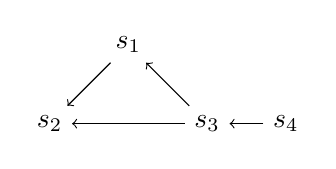
\begin{tikzpicture}
\node at (0,1) (a) {$s_1$};
\node at (1,0) (c)  {$s_3$};
\node at (-1,0) (b)  {$s_2$};
\node at (2,0) (d)  {$s_4$};

\draw[->] (a)->(b);
\draw[->] (c)->(a);
\draw[->] (c)->(b);
\draw[->] (d)->(c);
\end{tikzpicture}
}
\qquad\qquad
\begin{minipage}{1.2in}%

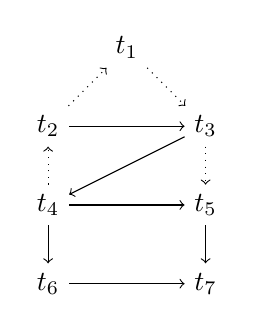
\begin{tikzpicture}
\node at (0,3) (alpha) {$t_1$};
\node at (-1,2) (beta)  {$t_2$};
\node at (1,2) (gamma)  {$t_3$};
\node at (-1,1) (delta)  {$t_4$};
\node at (1,1) (epsilon)  {$t_5$};
\node at (-1,0) (zeta)  {$t_6$};
\node at (1,0) (eta)  {$t_7$};

\draw[dotted, ->] (beta)->(alpha);
\draw[dotted, ->] (alpha)->(gamma);
\draw[->] (beta)->(gamma);
\draw[dotted, ->] (delta)->(beta);
\draw[->] (delta)->(epsilon);
\draw[->] (gamma)->(delta);
\draw[->] (epsilon)->(eta);
\draw[dotted, ->] (gamma)->(epsilon);
\draw[->] (zeta)->(eta);
\draw[->] (delta)->(zeta);

\end{tikzpicture}
\end{minipage}
\caption{Two graphs $G_1$ and $G_2$. $G_1$ is (node disjoint) subgraph homeomorphic to $G_2$ with the mapping $\{(s_1, t_5), (s_2, t_7), (s_3, t_4), (s_4, t_2), (s_1 \to s_2, t_5 \to t_7), (s_3 \to s_1, t_4 \to t_5), (s_3 \to s_2, t_4 \to t_6 \to t_7), (s_4 \to s_3, t_2 \to t_3 \to t_4)\}$. Other homeomorphisms exist as well.}
\end{figure}

If we have graphs $G_{virtual}$ and $G_{concrete}$, then wherever a subgraph homeomorphism from $G_{virtual}$ to $G_{concrete}$ exists, it describes a mapping where the logic of the virtual FPGA may be performed on the concrete FPGA in an emulation\footnote{If no such relation exists, it does not mean a function $f$ as specified in Section \ref{sec:Objectives} does not exist. Emulation could still be obtained by emulation of components by (multiple) components of possibly different types or by emulation of routing switches by sets of connected routing switches.}\footnote{This does not hold if some vertices in $G_{concrete}$ that are part of the mapping are unconfigurably connected and their mapped equivalents in $G_{virtual}$ are not. This is, however, rare and we account for this in our algorithm.}. The vertex-to-vertex mapping $\mathit{vmap}$ describes how to obtain configurations for the concrete FPGA and the edge-to-path mapping $\mathit{emap}$ describes how vertices in the concrete FPGA are connected via paths of intermediate components configured as wires.


The similarity between \textit{subgraph isomorphism} and \textit{subgraph homeomorphism} allows us to take inspiration from existing subgraph isomorphism algorithms and use similar methods to solve subgraph homeomorphism and therewith the FPGA emulation problem.

\subsection{Literature}
We performed literature research to obtain existing subgraph isomorphism and subgraph homeomorphism algorithms, the results of which are shown in Appendix \ref{app:algorithmHistory}. We searched the Scopus, ACM and IEEE libraries for the terms ``subgraph isomorphism", ``subgraph matching", ``subgraph homeomorphism" and ``topological minors". We examined matching papers and selected those that solve exact (not approximate) subgraph isomorphism or homeomorphism. We then iteratively added other algorithms from performance comparisons and citations. In the chart, an arrow implies that the paper of the newer algorithm or a survey paper showed that the algorithm at the source of the arrow performed better (i.e. lower mean time to find a matching) than the algorithm at the target of the arrow. A line between algorithms without arrowhead means a paper showed that the algorithms perform equally well.	


\subsubsection{Subgraph isomorhism}

Malik et al.\cite{Malik2019} simplify subgraph isomorphism by repeatedly randomly simplifying the target graph using a colouring.

PLGCoding\cite{Zhu2019}, based on LSGCoding\cite{Zhu20111272} uses the length of the shortest path and ``Laplacian spectra" to effectively index the target graph and search for subgraphs. However, the invariants that these methods use to solve subgraph isomorphism do not necessarily hold for subgraph homeomorphism.

subISO\cite{8711459} divides the target graph into subregions based on a pivot vertex in the pattern graph such that the number- and size of subregions is minimal. It then uses Ullmann\cite{ullmann1976} to search these subregions for the subgraph. Similarly, InfMatch\cite{Ma2019} uses heuristics to select a node in the target graph and selects subregions in the target graph from that node to search in. PTSim\cite{Xie2017} also applies graph partitioning, continuing with a different subgraph isomorphism algorithm on the resulting partitions, but only after first removing every edge from the target graph if the combination of labels of its source and target does not occur in the pattern graph. COSI\cite{5562766} uses partitioning of graphs in cloud networks to find subgraph queries in social network graphs. Afterwards, it uses L2G's algorithm\cite{Almasri2015}.

GRASS\cite{Bonnici2019}, a subgraph isomorphism algorithm for GPUs, solves the problem by iteratively alternating between DFS and BFS of partial matchings on GPU cells as deep as the GPU architecture allows. Since the search space of subgraph homeomorphism is much larger than that of subgraph isomorphism, this may cause problems on GPU cells with limited memory resources.

VF2++\cite{Juttner2018a} is an adaptation of VF2+\cite{Carletti2015}, an improvement on VF2\cite{Cordella2004} which in its turn is an improvement of VF\cite{906251}, a DFS algorithm in the search space of partial matchings in which the target graph is pruned using feasibility sets and the nodes in the pattern graph are matched in an efficient, fixed order. MuGram\cite{mugram} is a variation upon VF2 that allows multiple labels on each node. Since VF2++ has not been compared with RI-DS\cite{Bonnici2017}, it is unknown whether a fixed node order is a more promising technique than a dynamic node order.

RI\cite{RIalgorithm} is similarly to VF2++ a variant of DFS. It assigns a variable to each node in the pattern graph with the domain of possible matches in the target graph. In its DFS, it uses a \textit{dynamic} ordering of nodes. A node in the target graph is matched next if it has many neighbours in the existing partial matching, many neighbours of neighbours in the existing partial matching or else a large degree. With this, RI aims to maximize the number of verifiable constraints. RI-DS\cite{Bonnici2017} improves upon this by implementing a cache that checks label compatibility for nodes quicker. Rudolf\cite{rudolf} proposes a querying method to access graph data in a subgraph isomorphism problem within a constraint satisfaction problem context but does not provide an algorithm.

Similarly to RI, LAD\cite{LAD} solves subgraph isomorphism using constraints.  It then applies AllDifferent filtering (using an algorithm by Régin\cite{Regin1994362}) during constraint solving/DFS to reduce the domain as much as possible. This filtering removes every $u$ from the domain of $v$ whenever an assignment of $v$ to $u$ would result in an empty domain for some variable. McGregor\cite{MCGREGOR1979229} performs this as well but with a different AllDifferent algorithm. PathLAD\cite{Kotthoff2016} improves upon LAD by checking each match whether the number of 3-cycles of connected nodes in the target graph is at least as high as the number of 3-cycles in the pattern graph where it is matched. 

CLF-Match\cite{Bi2016} speeds up subgraph isomorphism by splitting the pattern graph into a dense core of well-connected nodes and sparse trees attached to it. By matching the core first, it avoids many unfruitful partial matches in DFS. Furthermore, it introduces a CPI data structure. This data structure helps to find subgraph isomorphisms more efficiently and takes polynomial time to construct.

LLAMA\cite{Kotthoff2016} and BM1\cite{Battiti2007} are portfolio techniques. Based on heuristics, they pick an approach from a collection that they expect to perform best. LLAMA picks from a collection of different algorithms whilst BM1 picks from different pruning settings for VF2.

BoostISO\cite{boostISO} introduces a filtering optimization for DFS: whenever a node $u$ in the pattern graph matches with a node $v$ in the target graph and it fails, any $v'$ in the target graph with a subset of the neighbours of $v$ will be disregarded as candidate match for $u$. It furthermore introduces a data structure that finds many subgraph isomorphisms as soon as one subgraph isomorphism is found.

Glassgow\cite{McCreesh2015} is a DFS algorithm with dynamic node ordering. Other than other often used filtering techniques to disregard potential matches, it introduces backjumping: whenever a finished recursive call fails to match a node $v$ in the source graph, it jumps back to the last time the domain of $v$ was changed. Furthermore, it introduces supplemental graphs: whenever a filter removes matches from the domain of a supplemental graph, it may also be removed from the domain of the original graph.

TurboISO\cite{Han2013} extracts subregions from the target graph by finding instances of a compressed tree (NEC) of the pattern graph in the target graph (a polynomial process). Furthermore, it proposes using the results of this DFS to generate a vertex order to be used in BFS for subgraph isomorphism.

SQBC\cite{ZHENG2014116} takes cliques into account when searching for subgraphs: any node in a maximal clique in the pattern graph needs to be matched with a node in a maximal clique in the target graph that is at least as large.

STW\cite{Sun2012788} splits the pattern graph into small pieces and attempts to find all occurrences of a graph piece. Within this set, it then iteratively searches for the next piece.


GraphQL\cite{graphql} filters the domain of source graph nodes based on the fact that neighbourhoods of nodes need to be sub-isomorphic to matched nodes in the target graph. It furthermore filters based on bijections from- and to adjacency subtrees. ILF \cite{Zampelli2010} formalizes this sub-isomorphism by iteratively strengthens the filtering power of labels until a fixed point indicates sub-isomorphisms. It uses these labels to reduce the domains of each source node and then updates labels to be as strong as possible.


NOVA\cite{Zhu2010140} computes for each node $v$ in the source vertex a \textit{signature}: for each node $u$ of distance $x < c$ it lists its label and the number of paths from $u$ to $v$ of length $x$. It uses this signature to filter out false matches from the domain of source graph nodes.

Treepi\cite{Zhang2007} and Gaddi\cite{gaddi} use the distances between node pairs to index graphs. Sing\cite{DiNatale2010} improves upon this by indexing the graph on the fly during the search process. SPath\cite{spath} also uses indexing techniques on trees and subgraphs to speed up the search for a complete mapping.

Subsea\cite{Lipets2009320} recursively cuts the target graph along its minimal cut, searches for the subgraph on the edges on this cut and the continues in the resulting two subregions. This algorithm assumes that a minimal cut has few edges and that the target graph is much larger than the source graph.

QuickSI\cite{QuickSI} makes use of a set of spanning entries to combine tree search with normal DFS.

Cheng\cite{CHENG1981371} proposes a method of storing constraints as matrices and performing matrix operations on Ullmann's\cite{ullmann1976} representation of partial mappings.

Ullmann\cite{ullmann1976} is often used as a baseline algorithm when testing subgraph isomorphism algorithms. It performs DFS using nodes with the highest degree in the source graph with random nodes in the target graph. L2G\cite{Almasri2015} improves upon this by selecting unassigned nodes from the target graph that are connected to the partial matching first. Fast-ON\cite{Gouda2012} improves upon Ullmann's algorithm by ordering the pattern graph vertices by degree and taking labels into account. UI\cite{Cibej2014} improves upon Ullmann's algorithm\cite{ullmann1976} by ordering the vertices of the pattern graph by a `subdegree' measure in descending order and by breaking ties by choosing the node with the highest closed-neighbourhood clustering value.

From this literature research, we conclude that a DFS for partial mappings is a viable approach to subgraph isomorphism and thus potential to subgraph homeomorphism. Many algorithms, however, use incompatible strategies to obtain subgraph isomorphisms. Experimentation will have to show what strategy is effective for path subgraph isomorphism.


\subsubsection{Subgraph Homeomorphism}
Lingas et al.\cite{LINGAS2009464} present an algorithm for subgraph homeomorphism under the assumption the vertex placement is fixed. For general subgraph homeomorphism they suggest trying their algorithm on each possible vertex matching.

Xiao et al.\cite{XIAONODEDISJOINT} present an algorithm for subgraph homeomorphism when the length of the intermediate paths is in a limited range\footnote{The algorithm involves precomputing all possible paths. The number of possible paths increases exponentially with the sizes of both the pattern- and target graph. Applying this to a graph model of an FPGA is infeasible.}. Since our path lengths can be $[1, +\infty)$, we would need to find an alternate solution.

Grohe et al.\cite{Grohe2011479} show that for every fixed source graph, an $O(|V_{target}|^3)$ algorithm exists that can find homeomorphic embeddings in any target graph. However, finding this algorithm is a non-trivial, NP-hard process.

LaPaugh et al.\cite{LaPaughOptim} present some ways to reduce the graphs in a subgraph homeomorphism problem. These reductions are, however, not applicable to FPGA graphs.


